% Provenance (never printed): old seconde/premiere S material on the water
% cycle on land (the drainage basin, river discharge, floods and their
% management); see sources/book2/PROVENANCE.md. The Varden basin is computed
% in figdata/grade-10/varden_basin.py from figdata/shared/region.py; the
% Potomac record in figdata/grade-10/flood_frequency.py.
\chapter{Bacias hidrográficas, rios e cheias}\label{ch:g10:drainage-basins}

Um rio pode subir dois dias depois que a chuva parou, numa cidade onde não
caiu chuva nenhuma. A água que inunda as suas ruas caiu antes, em morros
muito a montante; ela desceu pelas suas encostas até os córregos, e os
córregos se juntaram no rio que a trouxe, de uma só vez, até a cidade. Para
entender uma cheia, é preciso olhar além do rio, para toda a área que o
alimenta, e seguir a água através dela. Este capítulo define essa área, a
\omterm{def:g10:drainage-basins:drainage-basin}{bacia hidrográfica}; mede o que um rio transporta, a sua \omterm{def:g10:drainage-basins:discharge}{vazão}; acompanha uma
cheia enquanto ela passa por um ponto do rio; e mostra como um longo
registro de cheias diz com que frequência uma dada cheia volta.

\begin{omfigure}
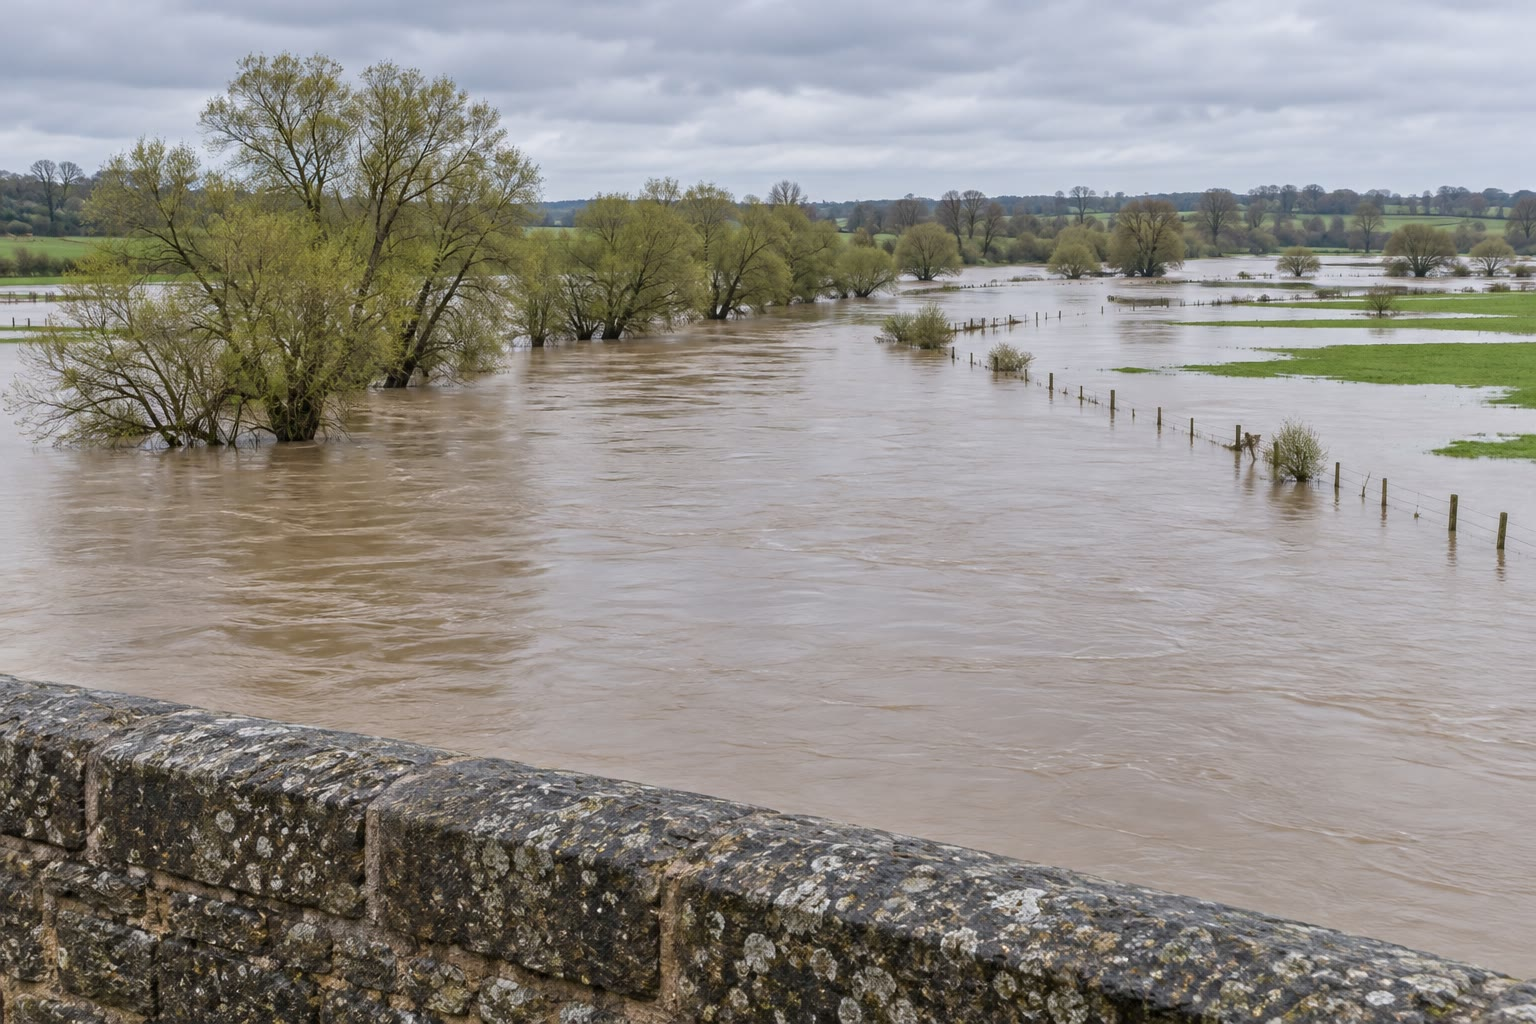
\includegraphics[width=0.8\linewidth]{images/book2/ai/g10-river-flood-meadows.jpg}

{\small Um rio em cheia, visto de uma ponte de pedra: a água marrom,
carregada de lama, saiu do seu leito e cobre os prados da sua planície de
inundação, até as cercas e as árvores que ladeiam as suas margens
habituais.}
\end{omfigure}

\begin{recall}
A chuva que chega ao chão se infiltra nele, escoa pela sua superfície ou se
evapora; o ciclo da água a leva de volta ao mar (os livros de física). A
água se infiltra nas rochas permeáveis e as enche abaixo do lençol freático,
formando aquíferos que alimentam fontes e rios (Livro 1, 6º ano). Um rio
serpenteia em meandros pela sua planície de inundação plana, que ele cobre
quando transborda (Livro 1, 5º ano). As curvas de nível unem pontos de mesma
altitude; as Colinas de Varden são a região desenhada nos mapas desta série
(Livro 1, 2º e 9º anos).
\end{recall}

\begin{safety}
A água de uma enchente é muito mais perigosa do que parece. Cerca de
\qty{15}{cm} de água correndo depressa podem derrubar um adulto, e cerca de
\qty{30}{cm} podem arrastar um carro; a estrada debaixo dela pode ter
desabado. Nunca entre a pé nem de carro na água de uma enchente: dê meia-volta
e vá por outro caminho.
% ledger: nws:flood-water
\end{safety}

\section{A bacia hidrográfica}

Cada gota de chuva que não evapora nem se infiltra fundo desce a encosta.
Ela segue o maior declive do terreno, junta-se a um filete, depois a um
córrego, e os córregos se juntam em rios. Toda a terra cuja água termina no
mesmo rio forma uma unidade.

\begin{definition}[Bacia hidrográfica; divisor de águas]\label{def:g10:drainage-basins:drainage-basin}
A \emph{bacia hidrográfica}\index{bacia hidrografica@bacia hidrográfica} de
um ponto de um rio é toda a área de terra cujo escoamento corre para o rio a
montante desse ponto e passa por esse ponto. O \emph{divisor de
águas}\index{divisor de aguas@divisor de águas} é a linha que separa duas
bacias hidrográficas vizinhas: ele segue as cristas do terreno, e a chuva
que cai de cada lado dele corre para rios diferentes.
\end{definition}

Uma bacia é sempre definida para um ponto do rio, o seu \emph{exutório}: a
bacia de um rio no ponto em que ele chega ao mar é a maior, e cada ponto a
montante tem uma bacia menor dentro dela. Duas gotas que caem a um metro uma
da outra, de cada lado de um divisor, podem terminar em rios diferentes e
até em oceanos diferentes.

\subsection*{A bacia do rio Varden}

Um computador encontra uma \omterm{def:g10:drainage-basins:drainage-basin}{bacia hidrográfica} a partir de um mapa de
altitudes em poucos passos. O mapa é cortado em pequenos quadrados, aqui de
\qty{50}{m} de lado. Para cada quadrado, o computador olha os seus oito
vizinhos e manda a água para aquele que é alcançado pelo maior declive
descendente. (Onde uma pequena depressão não tem vizinho mais baixo, ela é
primeiro preenchida até o nível em que transbordaria, como faz uma poça.)
Seguindo esses passos de quadrado em quadrado, traça-se o caminho de uma
gota a partir de qualquer ponto do mapa. Os quadrados cujas gotas chegam ao
rio formam a bacia.

\begin{omfigure}
\begin{tikzpicture}
\begin{axis}[axis equal image, xmin=0, xmax=10, ymin=0, ymax=8, width=0.86\linewidth,
  tick label style={font=\scriptsize}, xlabel={leste (km)}, ylabel={norte (km)},
  label style={font=\small}, enlargelimits=false]
\addplot[fill=omDef!14, draw=none, even odd rule] table {figdata/out/grade-10-varden_basin-fill.dat};
\addplot[contour, line width=0.25pt, opacity=0.7] table {figdata/out/shared-region-contours.dat};
\addplot[index contour, opacity=0.8] table {figdata/out/shared-region-index-contours.dat};
\addplot[river, line width=1.6pt] table {figdata/out/shared-region-river.dat};
\addplot[omThm, line width=1.4pt, dashed] table {figdata/out/grade-10-varden_basin-divide.dat};
\addplot[omWxRain, line width=0.9pt, -{Stealth[length=5pt]}] table {figdata/out/grade-10-varden_basin-path1.dat};
\addplot[omWxRain, line width=0.9pt, -{Stealth[length=5pt]}] table {figdata/out/grade-10-varden_basin-path2.dat};
\addplot[omWxRain, line width=0.9pt, -{Stealth[length=5pt]}] table {figdata/out/grade-10-varden_basin-path3.dat};
\addplot[omWxRain, line width=0.9pt, -{Stealth[length=5pt]}] table {figdata/out/grade-10-varden_basin-path4.dat};
\fill[omWxRain] (axis cs:2,7.4) circle (2.2pt);
\fill[omWxRain] (axis cs:4,1.8) circle (2.2pt);
\fill[omWxRain] (axis cs:8.6,6.6) circle (2.2pt);
\fill[omWxRain] (axis cs:2.5,0.7) circle (2.2pt);
\node[font=\footnotesize, fill=white, fill opacity=0.85, text opacity=1, inner sep=1.5pt, text=omThm] at (axis cs:6.0,6.75) {divisor};
\node[font=\footnotesize, fill=white, fill opacity=0.85, text opacity=1, inner sep=1.5pt, text=omThm] at (axis cs:3.5,1.1) {divisor};
\node[font=\footnotesize, fill=white, fill opacity=0.85, text opacity=1, inner sep=1.5pt, align=center] at (axis cs:5.3,7.55) {fora da bacia:\\a água sai para o norte};
\node[font=\footnotesize, fill=white, fill opacity=0.85, text opacity=1, inner sep=1.5pt, align=right, anchor=east] at (axis cs:9.85,3.35) {exutório};
\draw[-{Stealth[length=6pt]}, line width=1pt, omRiver] (axis cs:9.3,3.7) -- (axis cs:9.95,4.15);
\node[font=\footnotesize, fill=white, fill opacity=0.85, text opacity=1, inner sep=1.5pt] at (axis cs:1.1,4.75) {rio};
\end{axis}
\end{tikzpicture}

{\small A \omterm{def:g10:drainage-basins:drainage-basin}{bacia hidrográfica} do rio Varden no mapa das Colinas de Varden
(sombreada), calculada mandando a água de cada quadrado de \qty{50}{m} pelo
maior declive; curvas de nível a cada \qty{50}{m}. As linhas tracejadas são
os divisores; as linhas azuis são os caminhos de quatro gotas de chuva
(pontos). Duas chegam ao rio e correm para leste até o exutório, onde o rio
sai do mapa; as outras duas, além dos divisores, saem do mapa em direção a
outros rios.}
\end{omfigure}

A bacia cobre \qty{66}{km^2} dos \qty{80}{km^2} do mapa, cerca de quatro
quintos dele. No norte, o divisor segue as cristas dos morros e passa pelos
seus cumes; além deles, o terreno desce para longe do rio e a sua água corre
para outro vale. No canto sudoeste, uma pequena área também drena para fora
do mapa. O próprio rio entra no mapa pelo oeste, de modo que a sua bacia
completa é maior: ela inclui também a terra a montante, além da borda do
mapa.
% values computed in figdata/grade-10/varden_basin.py (basin_km2 66.19, map_km2 80)

\subsection*{Os maiores rios}

Os rios são comparados pela área da sua bacia e pela água que transportam.
O maior rio do mundo, de longe, é o Amazonas. O Mississippi, o maior rio dos
Estados Unidos, drena cerca de \num{1150000} milhas quadradas, cerca de 2.98
milhões de \unit{km^2}, dos Estados Unidos e do Canadá.
% ledger: kammerer:mississippi

\section{A vazão}

\begin{definition}[Vazão]\label{def:g10:drainage-basins:discharge}
A \emph{vazão}\index{vazao@vazão} de um rio num ponto é o volume de água que
atravessa uma seção transversal do rio em um segundo. Ela é medida em metros
cúbicos por segundo, \unit{m^3/s}.
\end{definition}

Uma \omterm{def:g10:drainage-basins:discharge}{vazão} de \qty{1}{m^3/s} são mil litros a cada segundo, ou
\qty{86400}{m^3} por dia. A água corre mais depressa perto da superfície, no
meio do canal, e mais devagar ao longo do leito e das margens, onde atrita
com eles; a \emph{velocidade média} é a velocidade calculada em média sobre
toda a seção transversal.

\begin{proposition}[Vazão, velocidade e seção transversal]\label{prop:g10:drainage-basins:discharge}
A \omterm{def:g10:drainage-basins:discharge}{vazão} $Q$ de um rio é o produto da velocidade média $v$ da água pela área
$A$ da seção molhada:
\[
Q = v\,A.
\]
\end{proposition}

\begin{proof}
Num tempo $t$, a água que atravessa a seção avançou uma distância $v\,t$:
ela enche uma fatia do rio de seção $A$ e comprimento $v\,t$, de volume
$A\,v\,t$. Dividindo esse volume pelo tempo $t$, obtém-se o volume por
segundo, $Q = v\,A$.
\end{proof}

Um rio com uma seção transversal de \qty{50}{m^2} que corre a uma velocidade
média de \qty{1.2}{m/s} transporta $1.2 \times 50 = \qty{60}{m^3/s}$. Na
cheia, os dois fatores crescem: a água fica mais funda e mais larga, de modo
que a seção cresce, e ela corre mais depressa.

\subsection*{Medir uma vazão}

Como a velocidade muda através do rio, ela é medida em vários pontos. O rio
é cortado em faixas verticais; em cada uma, medem-se a profundidade e a
velocidade, e somam-se as \omterm{def:g10:drainage-basins:discharge}{vazões} das faixas.

\begin{method}[O método velocidade--área]\label{met:g10:drainage-basins:velocity-area}
\begin{enumerate}
  \item Estique uma trena através do rio e escolha verticais a intervalos
        regulares $w$ ao longo dela.
  \item Em cada vertical, meça a profundidade $d$ e a velocidade média $v$
        da água nessa profundidade com um molinete.
  \item Cada vertical representa uma faixa de largura $w$ e área $w\,d$; a
        sua \omterm{def:g10:drainage-basins:discharge}{vazão} é $v\,w\,d$.
  \item Some as \omterm{def:g10:drainage-basins:discharge}{vazões} de todas as faixas: $Q = \sum v\,w\,d$.
        A seção transversal é $A = \sum w\,d$ e a velocidade média, $Q/A$.
\end{enumerate}
\end{method}

\begin{omfigure}
\begin{tikzpicture}[x=0.9cm, y=1.6cm, font=\footnotesize]
  % water
  \fill[omSea] (0,0) -- (1,-0.4) -- (2,-0.75) -- (3,-1.0) -- (4,-1.25) -- (5,-1.4) -- (6,-1.3)
     -- (7,-1.1) -- (8,-0.8) -- (9,-0.5) -- (10,-0.2) -- (10.5,0) -- cycle;
  \fill[omDef!22] (4,0) -- (4,-1.25) -- (5,-1.4) -- (6,-1.3) -- (6,0) -- cycle;
  % bed
  \draw[line width=0.9pt, brown!60!black] (-0.6,0.35) -- (0,0) -- (1,-0.4) -- (2,-0.75) -- (3,-1.0) -- (4,-1.25)
     -- (5,-1.4) -- (6,-1.3) -- (7,-1.1) -- (8,-0.8) -- (9,-0.5) -- (10,-0.2) -- (10.5,0) -- (11.1,0.35);
  \draw[omDef!70!black, line width=0.5pt] (0,0) -- (10.5,0);
  % verticals
  \foreach \x/\d/\v/\dx in {1/0.4/0.3/0.3, 3/1.0/0.6/0, 5/1.4/0.8/0, 7/1.1/0.7/0, 9/0.5/0.4/-0.25} {
    \draw[black!70, dashed] (\x,0) -- (\x,-\d);
    \node[anchor=south, font=\scriptsize] at (\x,0.02) {\qty{\v}{m/s}};
    \node[font=\scriptsize, fill=white, inner sep=0.8pt] at (\x+\dx,-0.5*\d) {\qty{\d}{m}};
  }
  \draw[{Stealth}-{Stealth}] (4,0.42) -- node[above, font=\scriptsize] {uma faixa: $w = \qty{2}{m}$} (6,0.42);
  \node[anchor=west, align=left] at (11.2,-0.15) {superfície\\da água};
  \node[anchor=west, align=left] at (11.2,-0.9) {leito};
  \draw[black!50] (11.15,-0.9) -- (8.5,-0.68);
  \node[anchor=north] at (5.25,-1.75) {velocidades médias medidas nas verticais (acima da água) e profundidades (na água)};
\end{tikzpicture}

{\small Medir uma \omterm{def:g10:drainage-basins:discharge}{vazão} (esquema; escala vertical exagerada). Cinco
verticais, a \qty{2}{m} umas das outras, dividem um córrego de cerca de
\qty{10}{m} de largura em faixas; a faixa sombreada é a medida na vertical
do meio.}
\end{omfigure}

\begin{example}[Uma medição de vazão]\label{ex:g10:drainage-basins:gauging}
No córrego da figura, as cinco faixas, cada uma com \qty{2}{m} de largura,
têm áreas $2 \times 0.4 = 0.8$, $2.0$, $2.8$, $2.2$ e \qty{1.0}{m^2}: a
seção transversal é de \qty{8.8}{m^2}. As suas \omterm{def:g10:drainage-basins:discharge}{vazões} são $0.3 \times 0.8 =
0.24$, $0.6 \times 2.0 = 1.20$, $0.8 \times 2.8 = 2.24$, $0.7 \times 2.2 =
1.54$ e $0.4 \times 1.0 = \qty{0.40}{m^3/s}$, de modo que o córrego
transporta $Q \approx \qty{5.6}{m^3/s}$. A velocidade média é $5.62/8.8 \approx
\qty{0.64}{m/s}$, menos que os \qty{0.8}{m/s} do meio do córrego.
\end{example}

\begin{omfigure}
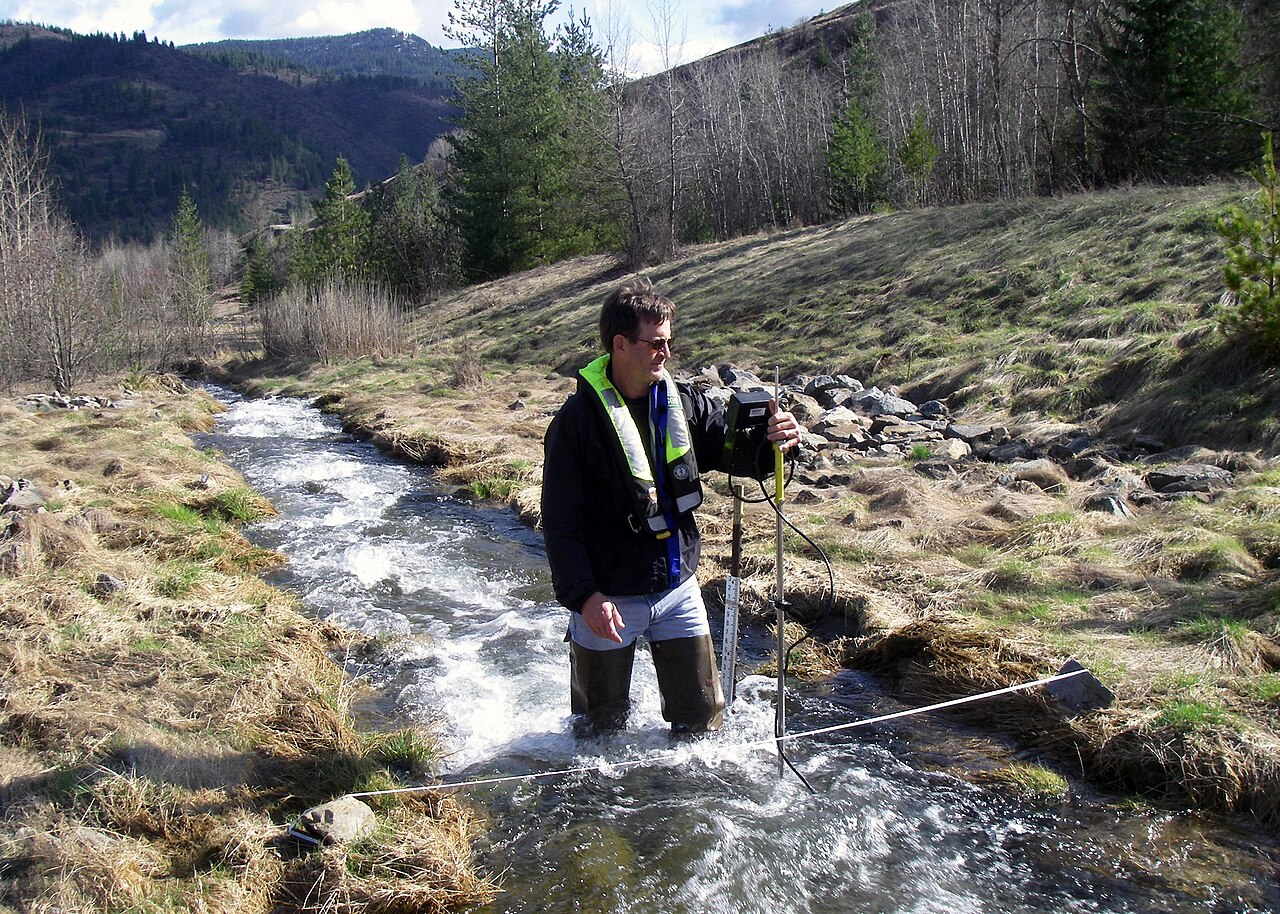
\includegraphics[height=4.6cm]{images/book2/g10-usgs-hydrologist-streamflow.jpg}\hspace{0.3cm}%
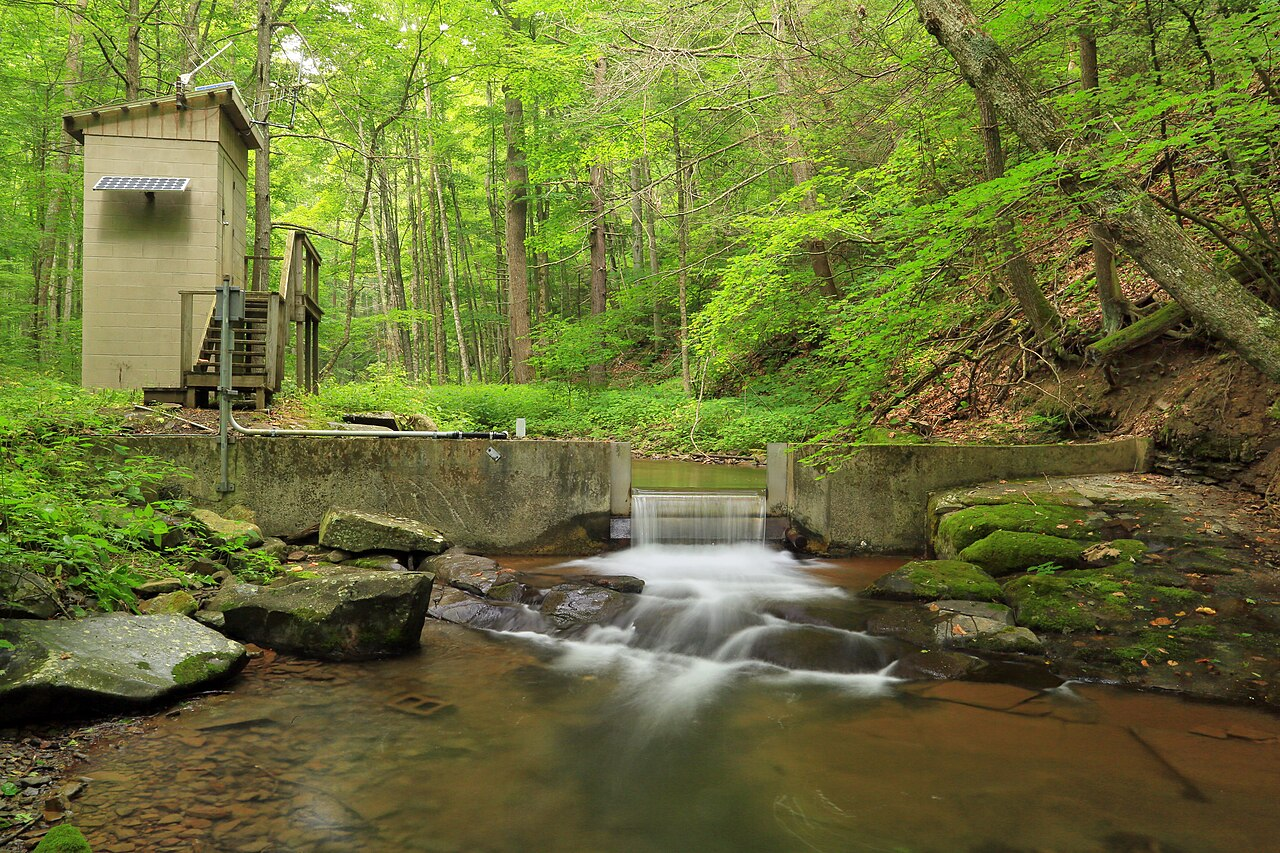
\includegraphics[height=4.6cm]{images/book2/g10-usgs-streamgage.jpg}

{\small À esquerda: uma hidróloga mede a \omterm{def:g10:drainage-basins:discharge}{vazão} de um córrego de montanha pelo
método velocidade--área; a trena esticada através do córrego marca as
verticais, e a haste leva um molinete. À direita: uma estação fluviométrica
num córrego de floresta; a cabana abriga os instrumentos que registram o
nível da água atrás do pequeno vertedouro. Fotografias: U.S. Geological
Survey (domínio público).}
\end{omfigure}

Uma medição de \omterm{def:g10:drainage-basins:discharge}{vazão} leva tempo e não pode ser feita continuamente. Uma
estação fluviométrica registra, em vez disso, o nível da água, sem
interrupção. Algumas medições feitas em níveis diferentes dão uma curva que
relaciona o nível à \omterm{def:g10:drainage-basins:discharge}{vazão}, e a estação converte cada nível que registra numa
\omterm{def:g10:drainage-basins:discharge}{vazão}.

Os grandes rios transportam \omterm{def:g10:drainage-basins:discharge}{vazões} enormes. De 1972 a 2003, o Amazonas
levou em média cerca de \qty{206000}{m^3/s} ao Oceano Atlântico, com uma
incerteza de cerca de \qty{6}{\percent}: cerca de \qty{17}{\percent} de toda
a água doce que os rios do mundo levam ao mar. O Mississippi leva em média
\num{593000} pés cúbicos por segundo, cerca de \qty{16800}{m^3/s}, ao Golfo
do México: o Amazonas transporta umas doze vezes mais.
% ledger: callede:amazon, kammerer:mississippi

\section{O hidrograma}

\begin{definition}[Hidrograma; escoamento de base; tempo de retardo]\label{def:g10:drainage-basins:hydrograph}
Um \emph{hidrograma}\index{hidrograma} é o gráfico da \omterm{def:g10:drainage-basins:discharge}{vazão} de um rio num
ponto em função do tempo. O \emph{escoamento de
base}\index{escoamento de base} é a parte da \omterm{def:g10:drainage-basins:discharge}{vazão} alimentada pela água subterrânea, que mantém o rio
correndo entre as chuvas. O \emph{tempo de retardo}\index{tempo de retardo}
de uma cheia é o tempo entre o pico da chuva sobre a bacia e o pico da
\omterm{def:g10:drainage-basins:discharge}{vazão}.
\end{definition}
\begin{omfigure}
\begin{tikzpicture}[x=1cm, y=1cm, font=\footnotesize]
  \draw[-{Stealth}] (0,0) -- (10.2,0) node[below left] {tempo};
  \draw[-{Stealth}] (0,0) -- (0,5.9) node[above right] {vazão};
  % rain bars hanging from the top
  \draw[black!50] (0,5.4) -- (10,5.4);
  \foreach \x/\h in {1.0/0.15, 1.3/0.35, 1.6/0.55, 1.9/0.4, 2.2/0.2} {
    \fill[omWxRain!70] (\x,5.4) rectangle ++(0.28,-\h);
  }
  \node[anchor=south west] at (2.6,5.4) {chuva sobre a bacia};
  % baseflow and hydrograph
  \fill[omSea] (0,0.7) -- (2.0,0.7) .. controls (2.8,0.8) and (3.3,3.3) .. (4.0,3.6)
    .. controls (4.6,3.6) and (5.1,2.1) .. (6.0,1.55) .. controls (7.0,1.0) and (8.0,0.85) .. (10,0.8)
    -- (10,0) -- (0,0) -- cycle;
  \fill[omLithAlluv] (0,0) -- (0,0.7) -- (2.0,0.7) .. controls (3.5,0.68) and (5.5,0.75) .. (6.6,0.95)
    .. controls (8,1.0) and (9,0.85) .. (10,0.8) -- (10,0) -- cycle;
  \draw[omDef, line width=1.2pt] (0,0.7) -- (2.0,0.7) .. controls (2.8,0.8) and (3.3,3.3) .. (4.0,3.6)
    .. controls (4.6,3.6) and (5.1,2.1) .. (6.0,1.55) .. controls (7.0,1.0) and (8.0,0.85) .. (10,0.8);
  \draw[black!60, dashed] (2.0,0.7) .. controls (3.5,0.68) and (5.5,0.75) .. (6.6,0.95);
  % lag time
  \draw[black!60, densely dotted] (1.74,4.85) -- (1.74,4.3);
  \draw[black!60, densely dotted] (3.98,3.65) -- (3.98,4.3);
  \draw[{Stealth}-{Stealth}] (1.74,4.3) -- node[above] {tempo de retardo} (3.98,4.3);
  % labels
  \node[anchor=west] at (4.2,3.75) {pico};
  \node[anchor=east, align=right] at (2.9,2.2) {ramo\\ascendente};
  \node[anchor=west, align=left] at (5.4,2.3) {ramo descendente};
  \node[align=center] at (4.5,1.25) {escoamento superficial};
  \node at (8.2,0.4) {escoamento de base};
\end{tikzpicture}

{\small O \omterm{def:g10:drainage-basins:hydrograph}{hidrograma} de uma cheia (esquema). Depois da chuva, a \omterm{def:g10:drainage-basins:discharge}{vazão} sobe
até um pico e volta a cair mais devagar; a área sob a curva é o volume de
água. O \omterm{def:g10:drainage-basins:hydrograph}{escoamento de base}, alimentado pela água subterrânea, muda pouco; o
resto é o escoamento superficial que a chuva mandou depressa para o rio.}
\end{omfigure}

A água de uma tempestade chega ao rio em momentos diferentes. A chuva que cai
perto do canal chega em minutos ou horas; a chuva que cai muito a montante
leva muito mais tempo, já que precisa descer pelas encostas e ao longo do
rio. A \omterm{def:g10:drainage-basins:discharge}{vazão}, portanto, sobe abruptamente, no \emph{ramo ascendente},
enquanto chega a água das encostas próximas, atinge o pico quando a maior
quantidade de água chega de uma vez, e cai mais devagar, no \emph{ramo
descendente}, à medida que a última água escoa dos cantos distantes da
bacia e do solo. Quanto maior a bacia, mais longo o \omterm{def:g10:drainage-basins:hydrograph}{tempo de retardo}: horas
para um pequeno córrego, dias para um grande rio.

Algumas bacias dão cheias \emph{repentinas}, com um pico alto e súbito e um
\omterm{def:g10:drainage-basins:hydrograph}{tempo de retardo} curto; outras dão cheias lentas e achatadas. A mesma chuva
dá uma cheia mais repentina quando:
\begin{itemize}
  \item a bacia é pequena e íngreme, de modo que a água tem um caminho curto
        e rápido a percorrer;
  \item o terreno deixa pouca água se infiltrar: rocha nua, argila, terreno
        já encharcado, terreno congelado e, sobretudo, os telhados, as ruas
        e os estacionamentos de uma cidade, que mandam quase toda a chuva
        direto para os bueiros e os córregos;
  \item a bacia tem uma rede densa de córregos e de galerias, que recolhe a
        água depressa.
\end{itemize}
As florestas, os solos profundos e permeáveis e as planícies de inundação
largas fazem o contrário: elas retêm a água e a liberam devagar, o que
abaixa e atrasa o pico.

\subsection*{Uma cheia real}

O rio Potomac drena uma bacia de \num{11560} milhas quadradas, cerca de
\qty{29900}{km^2}, a montante de uma estação fluviométrica perto de
Washington, no leste dos Estados Unidos. Em janeiro de 1996, a estação
registrou o \omterm{def:g10:drainage-basins:hydrograph}{hidrograma} abaixo.
% ledger: data:b2-usgs-potomac

\begin{omfigure}
\begin{tikzpicture}
\begin{axis}[omrecord, width=0.86\linewidth, height=6cm, xmin=0, xmax=55, ymin=0, ymax=10000,
  xtick={0,10,20,30,40,50}, xticklabels={5 jan., 15 jan., 25 jan., 4 fev., 14 fev., 24 fev.},
  ylabel={vazão (\unit{m^3/s})}, xlabel={1996},
  tick label style={font=\small}, label style={font=\small},
  scaled y ticks=false, yticklabel style={/pgf/number format/fixed}]
\addplot[omDef, line width=1.1pt, mark=*, mark size=1.1pt] table[x=day, y=q] {figdata/out/grade-10-flood_frequency-hydrograph.dat};
\node[anchor=west, font=\footnotesize] at (axis cs:17,9231) {\qty{9231}{m^3/s} em 21 de janeiro};
\draw[black!60, dashed] (axis cs:5,334) -- (axis cs:13,334);
\node[anchor=south, font=\footnotesize] at (axis cs:9,1000) {uns \qty{330}{m^3/s}};
\draw[black!60] (axis cs:9,1000) -- (axis cs:9,390);
\end{axis}
\end{tikzpicture}

{\small \omterm{def:g10:drainage-basins:discharge}{Vazão} média diária do rio Potomac perto de Washington de 5 de
janeiro a 29 de fevereiro de 1996: a cheia subiu de \qty{362}{m^3/s} em 18
de janeiro para mais de \qty{9000}{m^3/s} três dias depois, e depois voltou
a cair nas semanas seguintes, com uma segunda subida menor no fim de
janeiro. Dados: U.S. Geological Survey, estação 01646500.}
\end{omfigure}
% values computed in figdata/grade-10/flood_frequency.py (hydro_peak_m3s 9231, hydro_before_mean 334)

Nos dias antes da cheia, o rio transportava cerca de \qty{330}{m^3/s}, o seu
\omterm{def:g10:drainage-basins:hydrograph}{escoamento de base}. Em 21 de janeiro, a média diária chegou a
\qty{9231}{m^3/s}, quase trinta vezes mais. Espalhada sobre toda a bacia, a
água que passou pela estação nesse dia formaria uma camada de
$9231 \times 86400 / (29\,900 \times 10^6) \approx \qty{0.027}{m}$, cerca de
\qty{27}{mm} de profundidade: uma chuva forte, entregue em um dia pela bacia
inteira ao mesmo tempo.
% ledger: data:b2-usgs-potomac (hydro_peak_mm_per_day 26.6 in figdata/grade-10/flood_frequency.py)

\section{As cheias e o seu período de retorno}

Que tamanho de cheia uma cidade deve esperar? A resposta vem do passado: uma
estação fluviométrica que funciona há décadas registrou a maior \omterm{def:g10:drainage-basins:discharge}{vazão} de
cada ano, o \emph{pico anual}. Picos pequenos vêm quase todo ano, os grandes
raramente. Quanto mais rara uma cheia, maior ela é.

\begin{definition}[Período de retorno]\label{def:g10:drainage-basins:return-period}
O \emph{período de retorno}\index{periodo de retorno@período de retorno} $T$
de uma cheia é o intervalo médio, em anos, entre os anos cujo pico anual a
iguala ou a supera. Uma cheia de período de retorno $T$, uma \emph{cheia de
$T$ anos}, tem uma probabilidade $1/T$ de ser igualada ou superada num ano
qualquer.
\end{definition}

Uma cheia de cem anos não é uma cheia que vem uma vez a cada cem anos, como
num horário. É uma cheia que tem uma chance em cem de ser igualada ou
superada a cada ano, todo ano, aconteça o que tiver acontecido no ano
anterior. Duas podem vir em anos seguidos; um século pode passar sem
nenhuma.

\begin{method}[Os períodos de retorno a partir de um registro de picos anuais]\label{met:g10:drainage-basins:return-periods}
\begin{enumerate}
  \item Liste os picos anuais de $n$ anos.
  \item Ordene-os do maior (posto $m = 1$) ao menor (posto $m = n$).
  \item Atribua ao pico de posto $m$ o \omterm{def:g10:drainage-basins:return-period}{período de retorno} $T = (n + 1)/m$.
  \item Represente os picos em função de $T$ numa escala logarítmica de $T$,
        e leia a \omterm{def:g10:drainage-basins:discharge}{vazão} para o \omterm{def:g10:drainage-basins:return-period}{período de retorno} desejado.
\end{enumerate}
\end{method}

O maior de $n$ picos recebe, assim, $T = n + 1$ anos: num registro de
\num{95} anos, \num{96} anos. A fórmula reflete o que o registro mostra: o
pico de posto $m$ foi igualado ou superado em $m$ dos $n$ anos, cerca de uma
vez a cada $n/m$ anos. O método não consegue ir, de forma confiável, além da
duração do registro: um registro de \num{50} anos diz pouco sobre a cheia de
\num{1000} anos.

\begin{omfigure}
\begin{tikzpicture}
\begin{axis}[omrecord, width=0.86\linewidth, height=6.2cm, xmode=log, xmin=0.9, xmax=150,
  ymin=0, ymax=15000, xlabel={período de retorno $T$ (anos)}, ylabel={pico anual (\unit{m^3/s})},
  xtick={1,2,5,10,20,50,100}, xticklabels={1,2,5,10,20,50,100},
  tick label style={font=\small}, label style={font=\small},
  scaled y ticks=false, yticklabel style={/pgf/number format/fixed}]
\addplot[only marks, mark=*, mark size=1.5pt, omDef] table[x=T, y=peak] {figdata/out/grade-10-flood_frequency-ranked.dat};
\node[anchor=east, font=\footnotesize] at (axis cs:92,13705) {1936};
\node[anchor=east, font=\footnotesize] at (axis cs:46,12658) {1942};
\node[anchor=south, font=\footnotesize] at (axis cs:32,10300) {1972};
\node[anchor=north west, font=\footnotesize, align=left] at (axis cs:1.1,14000) {rio Potomac perto de Washington,\\picos anuais 1931--2025 ($n = 95$)};
\end{axis}
\end{tikzpicture}

{\small Os \num{95} picos anuais do rio Potomac perto de Washington,
ordenados e representados em função dos seus \omterm{def:g10:drainage-basins:return-period}{períodos de retorno}
$T = (n+1)/m$. O maior, em março de 1936, recebe $T = 96$ anos. Dados: U.S.
Geological Survey, estação 01646500.}
\end{omfigure}
% values computed in figdata/grade-10/flood_frequency.py

\begin{dated}{2026}
No registro do Potomac perto de Washington, de 1931 a 2025, os cinco maiores
picos anuais ocorreram em março de 1936 (\qty{13700}{m^3/s}), outubro de
1942, junho de 1972, abril de 1937 e janeiro de 1996, os dois últimos iguais
a \qty{9830}{m^3/s}.
% ledger: data:b2-usgs-potomac
\end{dated}

\subsection*{A chance de uma cheia ao longo de muitos anos}

Uma casa ou uma ponte fica de pé durante décadas. O que importa para ela não
é a chance de uma cheia num ano, mas ao longo de toda a sua vida.

\begin{proposition}[Pelo menos uma cheia em $N$ anos]\label{prop:g10:drainage-basins:chance}
Se os anos são independentes uns dos outros, a probabilidade de que uma
cheia de \omterm{def:g10:drainage-basins:return-period}{período de retorno} $T$ seja igualada ou superada pelo menos uma vez
em $N$ anos é
\[
P = 1 - \left(1 - \frac{1}{T}\right)^{N}.
\]
\end{proposition}

\begin{proof}
Num ano, a probabilidade de que a cheia \emph{não} aconteça é $1 - 1/T$.
Sendo os anos independentes, a probabilidade de que ela não aconteça em
nenhum dos $N$ anos é o produto de $N$ fatores desses, $(1 - 1/T)^N$. O
evento ``pelo menos uma vez'' é o contrário de ``nunca'', logo a sua
probabilidade é $1 - (1 - 1/T)^N$.
\end{proof}

Para uma cheia de cem anos ao longo de trinta anos,
$(0.99)^{30} \approx 0.740$, e $P \approx 0.26$: uma chance em quatro. Ao longo de cem anos, $(0.99)^{100}
\approx 0.366$ e $P \approx 0.63$: está longe de ser certo que
a cheia de cem anos venha em cem anos.

\begin{omfigure}
\begin{tikzpicture}
\begin{axis}[omrecord, width=0.82\linewidth, height=5.8cm, xmin=0, xmax=100, ymin=0, ymax=1,
  xlabel={número de anos $N$}, ylabel={chance de pelo menos uma cheia},
  ytick={0,0.2,0.4,0.6,0.8,1}, yticklabels={0, 20\,\%, 40\,\%, 60\,\%, 80\,\%, 100\,\%},
  tick label style={font=\small}, label style={font=\small},
  legend pos=south east, legend style={font=\footnotesize}]
\addplot[omThm, line width=1pt] table[x=n, y=p10] {figdata/out/grade-10-flood_frequency-chance.dat};
\addplot[omProp, line width=1pt] table[x=n, y=p50] {figdata/out/grade-10-flood_frequency-chance.dat};
\addplot[omDef, line width=1pt] table[x=n, y=p100] {figdata/out/grade-10-flood_frequency-chance.dat};
\legend{{cheia de 10 anos}, {cheia de 50 anos}, {cheia de 100 anos}}
\draw[black!60, dashed] (axis cs:30,0) -- (axis cs:30,0.2603) -- (axis cs:0,0.2603);
\fill[omDef] (axis cs:30,0.2603) circle (2pt);
\node[anchor=north west, font=\footnotesize] at (axis cs:31,0.22) {26\,\% em 30 anos};
\end{axis}
\end{tikzpicture}

{\small A chance de que uma cheia de \omterm{def:g10:drainage-basins:return-period}{período de retorno} 10, 50 ou 100 anos
venha pelo menos uma vez em $N$ anos.}
\end{omfigure}
% values computed in figdata/grade-10/flood_frequency.py (chance_100_30 0.2603)

\section{Barragens e diques}

Há muito tempo as pessoas constroem estruturas que mudam a maneira como uma
cheia passa. Duas delas a mudam de modos opostos.

Uma \emph{barragem} retém um reservatório. Quando chega uma cheia, parte da
sua água é armazenada no reservatório, cujo nível sobe, e é liberada depois,
ao longo de um tempo maior. A jusante, passa o mesmo volume de água, mas
espalhado: o pico é mais baixo e mais tardio. Um reservatório só abaixa uma
cheia enquanto ainda tem espaço livre; uma vez cheio, toda a água que entra
nele segue adiante.

Um \emph{dique} é um aterro de terra construído ao longo de um rio para
manter as suas cheias fora da planície de inundação. Entre os diques, a água
não consegue se espalhar; para transportar a mesma \omterm{def:g10:drainage-basins:discharge}{vazão} pela seção mais
estreita, ela precisa ficar mais alta e correr mais depressa. A terra atrás
dos diques fica seca, enquanto os diques resistirem e não forem
transbordados. Mas a planície de inundação não armazena mais água durante a
cheia, de modo que mais água, e mais cedo, desce o rio.

\begin{omfigure}
\begin{tikzpicture}[x=0.62cm, y=0.62cm, font=\footnotesize]
  \begin{scope}
    \draw[-{Stealth}] (0,0) -- (9.4,0) node[below left] {tempo};
    \draw[-{Stealth}] (0,0) -- (0,6.0) node[above right] {vazão};
    \draw[omDef, line width=1.2pt] (0,0.6) -- (1,0.6) .. controls (1.8,0.7) and (2.2,5.2) .. (2.8,5.2)
      .. controls (3.5,5.2) and (4,1.6) .. (5,1.0) .. controls (6,0.7) and (7.5,0.6) .. (9,0.6);
    \draw[omThm, line width=1.2pt, dashed] (0,0.6) -- (1.3,0.6) .. controls (2.3,0.75) and (3.0,3.3) .. (3.8,3.3)
      .. controls (4.7,3.3) and (5.8,1.5) .. (6.8,1.0) .. controls (7.6,0.75) and (8.3,0.65) .. (9,0.6);
    \node[anchor=west, text=omDef] at (3.0,5.35) {entrando no reservatório};
    \node[anchor=west, text=omThm] at (4.2,3.55) {abaixo da barragem};
    \node[anchor=north] at (4.5,-0.45) {(a) uma barragem: pico mais baixo e mais tardio};
  \end{scope}
  \begin{scope}[xshift=7.2cm]
    \fill[omLithAlluv] (0,0) -- (10,0) -- (10,1.8) -- (0,1.8) -- cycle;
    \fill[white] (3.5,1.8) -- (3.9,0.4) -- (6.1,0.4) -- (6.5,1.8) -- cycle;
    \fill[omSea] (0.4,2.3) -- (3.25,2.3) -- (3.5,1.8) -- (3.9,0.4) -- (6.1,0.4) -- (6.5,1.8) -- (6.75,2.3) -- (9.6,2.3) -- (9.6,1.8) -- (0.4,1.8) -- cycle;
    \draw[line width=0.8pt, brown!60!black] (0,1.8) -- (3.5,1.8) -- (3.9,0.4) -- (6.1,0.4) -- (6.5,1.8) -- (10,1.8);
    \draw[omDef!70!black] (0.4,2.3) -- (9.6,2.3);
    \node[anchor=south, text=omDef!70!black, align=center] at (1.5,2.35) {sem\\diques};
    % levees
    \fill[brown!45] (2.6,1.8) -- (3.0,3.9) -- (3.3,3.9) -- (3.5,1.8) -- cycle;
    \fill[brown!45] (6.5,1.8) -- (6.7,3.9) -- (7.0,3.9) -- (7.4,1.8) -- cycle;
    \fill[omSea!70!omDef] (3.5,1.8) -- (3.9,0.4) -- (6.1,0.4) -- (6.5,1.8) -- (6.65,3.4) -- (3.35,3.4) -- cycle;
    \draw[omThm, line width=0.8pt, dashed] (3.35,3.4) -- (6.65,3.4);
    \node[anchor=south, text=omThm] at (5,3.95) {com diques};
    \draw[omThm] (5,3.95) -- (5,3.45);
    \node[anchor=north] at (5,-0.45) {(b) diques: a cheia fica mais alta};
  \end{scope}
\end{tikzpicture}

{\small Esquema. (a) Um reservatório armazena parte de uma cheia e a libera
mais tarde: abaixo da barragem, o pico é mais baixo e vem mais tarde. (b)
Sem diques, a cheia se espalha numa lâmina fina sobre a planície de
inundação; entre diques, a mesma \omterm{def:g10:drainage-basins:discharge}{vazão} precisa passar por uma seção estreita
e fica muito mais alta.}
\end{omfigure}

\section{Exercícios}

\begin{exercise}[$\star$]\label{exo:g10:drainage-basins:1}
Defina uma \omterm{def:g10:drainage-basins:drainage-basin}{bacia hidrográfica} e um \omterm{def:g10:drainage-basins:drainage-basin}{divisor de águas}. Por que duas gotas de
chuva que caem a um metro uma da outra podem terminar em dois mares
diferentes?
\end{exercise}

\begin{exercise}[$\star$]\label{exo:g10:drainage-basins:2}
Defina a \omterm{def:g10:drainage-basins:discharge}{vazão} de um rio e dê a sua unidade. Quantos litros passam em um dia
por um ponto de um rio que transporta \qty{1}{m^3/s}?
\end{exercise}

\begin{exercise}[$\star$]\label{exo:g10:drainage-basins:3}
No \omterm{def:g10:drainage-basins:hydrograph}{hidrograma} do Potomac de janeiro de 1996, leia o \omterm{def:g10:drainage-basins:hydrograph}{escoamento de base} antes
da cheia, a \omterm{def:g10:drainage-basins:discharge}{vazão} de pico e a sua data, e o número de dias que a subida
levou.
\end{exercise}

\begin{exercise}[$\star$]\label{exo:g10:drainage-basins:4}
Qual é a probabilidade de que uma cheia de \num{50} anos seja igualada ou
superada no ano que vem? Uma cheia de \num{50} anos veio no ano passado: ela
é menos provável neste ano?
\end{exercise}

\begin{exercise}[$\star$]\label{exo:g10:drainage-basins:5}
O Mississippi leva em média \num{593000} pés cúbicos de água por segundo ao
mar (\num{1}~pé = \qty{0.3048}{m}). Converta essa \omterm{def:g10:drainage-basins:discharge}{vazão} em \unit{m^3/s} e
compare-a com os \qty{206000}{m^3/s} do Amazonas.
\end{exercise}

\begin{exercise}[$\star\star$]\label{exo:g10:drainage-basins:6}
Uma hidróloga mede a \omterm{def:g10:drainage-basins:discharge}{vazão} de um córrego com quatro verticais a
\qty{1.5}{m} umas das outras. As profundidades são \num{0.3}, \num{0.6},
\num{0.7} e \qty{0.4}{m}; as velocidades médias, \num{0.2}, \num{0.5},
\num{0.6} e \qty{0.3}{m/s}. Calcule a seção transversal, a \omterm{def:g10:drainage-basins:discharge}{vazão} e a
velocidade média.
\end{exercise}

\begin{exercise}[$\star\star$]\label{exo:g10:drainage-basins:7}
Uma tempestade despeja \qty{20}{mm} de chuva sobre toda a bacia do rio
Varden no mapa, \qty{66}{km^2}. Que volume de água é esse? Se toda ela
chegasse ao exutório em dois dias, qual seria a \omterm{def:g10:drainage-basins:discharge}{vazão} extra média?
\end{exercise}

\begin{exercise}[$\star\star$]\label{exo:g10:drainage-basins:8}
Os picos anuais de um pequeno rio ao longo de nove anos são, em
\unit{m^3/s}: \num{42}, \num{65}, \num{38}, \num{120}, \num{51}, \num{47},
\num{88}, \num{35}, \num{59}. Ordene-os e dê os \omterm{def:g10:drainage-basins:return-period}{períodos de retorno} dos três
maiores. Qual é o \omterm{def:g10:drainage-basins:return-period}{período de retorno} do pico mediano?
\end{exercise}

\begin{exercise}[$\star\star$]\label{exo:g10:drainage-basins:9}
A mesma tempestade cai sobre duas bacias de mesma área: uma íngreme, coberta
por uma cidade, a outra de declive suave e coberta de floresta. Esboce os
seus dois \omterm{def:g10:drainage-basins:hydrograph}{hidrogramas} nos mesmos eixos e explique as diferenças.
\end{exercise}

\begin{exercise}[$\star\star$]\label{exo:g10:drainage-basins:10}
No pico de 21 de janeiro de 1996, o Potomac transportava \qty{9231}{m^3/s}
de uma bacia de \qty{29900}{km^2}. Que lâmina de água, espalhada sobre toda
a bacia, representa um dia dessa \omterm{def:g10:drainage-basins:discharge}{vazão}? Compare com o \omterm{def:g10:drainage-basins:hydrograph}{escoamento de base} de
\qty{330}{m^3/s}.
\end{exercise}

\begin{exercise}[$\star\star$]\label{exo:g10:drainage-basins:11}
Qual é a probabilidade de que uma cheia de \num{10} anos venha pelo menos
uma vez em \num{10} anos? E de que ela não venha nenhuma vez nesses dez anos?
\end{exercise}

\begin{exercise}[$\star\star\star$]\label{exo:g10:drainage-basins:12}
A \omterm{def:g10:drainage-basins:discharge}{vazão} que entra num reservatório durante uma cheia sobe regularmente de
\qty{0}{m^3/s} a \qty{1200}{m^3/s} em um dia, e depois cai regularmente de
volta a \qty{0}{m^3/s} em dois dias (\omterm{def:g10:drainage-basins:hydrograph}{escoamento de base} desprezado). Que
volume a cheia traz? A barragem deixa passar no máximo \qty{800}{m^3/s}, e
o reservatório pode armazenar \num{60} milhões de \unit{m^3}. Ele consegue
reter tudo o que passa de \qty{800}{m^3/s}?
\end{exercise}

\begin{exercise}[$\star\star\star$]\label{exo:g10:drainage-basins:13}
Um rio de \qty{100}{m} de largura está cheio até as margens com
\qty{800}{m^3/s}, correndo a \qty{2}{m/s}. Chega uma cheia de
\qty{1200}{m^3/s}.
\begin{enumerate}
  \item Sem diques, os \qty{400}{m^3/s} extras se espalham por uma planície
        de inundação de \qty{900}{m} de largura, onde correm a
        \qty{0.5}{m/s}. Qual é a profundidade da água na planície de
        inundação?
  \item Com diques, toda a cheia passa entre eles, a \qty{2}{m/s}. Qual é a
        profundidade do rio, e a que altura acima das suas margens ele
        fica?
\end{enumerate}
\end{exercise}

\begin{exercise}[$\star\star\star$]\label{exo:g10:drainage-basins:14}
Que \omterm{def:g10:drainage-basins:return-period}{período de retorno} $T$ dá a uma cheia uma chance em duas de vir pelo
menos uma vez em \num{30} anos?
\end{exercise}

\begin{exercise}[$\star\star\star$]\label{exo:g10:drainage-basins:15}
Um pequeno mapa é cortado em quadrados de \qty{100}{m}; as suas altitudes em
metros são dadas abaixo (norte em cima). A água sai de cada quadrado em
direção ao mais baixo dos seus quatro vizinhos (norte, sul, leste, oeste),
se ele for mais baixo; os quadrados a \qty{34}{m} (canto noroeste) e a
\qty{30}{m} (canto sudeste) são os exutórios de dois córregos.
\begin{center}
\begin{tabular}{|c|c|c|c|}
\hline
34 & 38 & 46 & 50 \\ \hline
37 & 42 & 48 & 47 \\ \hline
45 & 49 & 44 & 39 \\ \hline
51 & 46 & 37 & 30 \\ \hline
\end{tabular}
\end{center}
Desenhe a direção do escoamento de cada quadrado, encontre a bacia de cada
exutório e a sua área, e desenhe o divisor.
\end{exercise}

\section{Problema: a cheia de cem anos}

\begin{problem}[{Problema de fim de semana --- com que frequência o rio entra na cidade?}]
\label{pb:g10:drainage-basins:1}
% ledger: data:b2-usgs-potomac (values computed in figdata/grade-10/flood_frequency.py)
Imagine uma cidade às margens do rio Potomac, logo a montante de Washington,
perto de uma estação fluviométrica que registrou a maior \omterm{def:g10:drainage-basins:discharge}{vazão} do rio a cada
ano desde 1931. Os picos anuais estão desenhados abaixo, e o \omterm{def:g10:drainage-basins:hydrograph}{hidrograma} de
janeiro de 1996 foi dado no capítulo.

\begin{center}
\begin{tikzpicture}
\begin{axis}[omrecord, width=0.9\linewidth, height=5.4cm, ybar, bar width=1.6pt, xmin=1929, xmax=2027,
  ymin=0, ymax=15000, ylabel={pico anual (\unit{m^3/s})}, xlabel={ano},
  xtick={1930,1950,1970,1990,2010}, xticklabel style={/pgf/number format/1000 sep={}},
  tick label style={font=\small}, label style={font=\small},
  scaled y ticks=false, yticklabel style={/pgf/number format/fixed}]
\addplot[fill=omDef!70, draw=none] table[x=year, y=peak] {figdata/out/grade-10-flood_frequency-record.dat};
\draw[omThm, dashed] (axis cs:1929,9500) -- (axis cs:2027,9500);
\node[anchor=south east, font=\footnotesize, text=omThm] at (axis cs:2026,9500) {\qty{9500}{m^3/s}};
\end{axis}
\end{tikzpicture}

{\small Picos anuais de \omterm{def:g10:drainage-basins:discharge}{vazão} do rio Potomac perto de Washington, anos
hidrológicos 1931--2025 (um ano hidrológico vai de outubro a setembro: a
cheia de outubro de 1942 conta em 1943). Dados: U.S. Geological Survey,
estação 01646500.}
\end{center}

\medskip
\noindent\textbf{Parte I --- A bacia e a vazão.}
\begin{enumerate}
  \item A bacia da estação cobre \num{11560} milhas quadradas
        (\num{1}~milha = \qty{1.609}{km}). Converta essa área em
        \unit{km^2}.
  \item Que linha, num mapa, limita essa área?
  \item O maior pico, em 19 de março de 1936, foi de \num{484000} pés
        cúbicos por segundo. Converta-o em \unit{m^3/s} (\num{1}~pé =
        \qty{0.3048}{m}).
  \item O pico anual mediano é de \qty{3341}{m^3/s}. Quantas vezes maior que
        a mediana foi a cheia de 1936?
  \item Suponha que, no pico de 1936, o rio tivesse \qty{400}{m} de largura
        e \qty{8}{m} de profundidade média na estação. Qual teria sido a sua
        velocidade média?
\end{enumerate}

\medskip
\noindent\textbf{Parte II --- Ler a cheia de 1996.}
\begin{enumerate}[resume]
  \item No \omterm{def:g10:drainage-basins:hydrograph}{hidrograma} de janeiro de 1996, qual era o \omterm{def:g10:drainage-basins:hydrograph}{escoamento de base} nos
        dias antes da cheia?
  \item Qual foi a \omterm{def:g10:drainage-basins:discharge}{vazão} diária de pico, e em que dia?
  \item Quantos dias a subida levou, de \qty{362}{m^3/s} em 18 de janeiro
        até o pico?
  \item Que lâmina de água sobre toda a bacia o dia do pico fez passar pela
        estação?
  \item Uma segunda subida, menor, atinge o pico em 29 de janeiro. O que ela
        diz sobre a água que chega à bacia?
  \item A \omterm{def:g10:drainage-basins:discharge}{vazão} voltou para perto de \qty{410}{m^3/s} em 7 de fevereiro.
        Quanto tempo depois do pico foi isso? Por que o ramo descendente
        dura mais que o ramo ascendente?
\end{enumerate}

\medskip
\noindent\textbf{Parte III --- Ordenar as cheias.}
\begin{enumerate}[resume]
  \item O registro contém $n = 95$ picos anuais. Que \omterm{def:g10:drainage-basins:return-period}{período de retorno} o
        método dá ao maior?
  \item O pico de outubro de 1942 (\qty{12658}{m^3/s}) está em segundo
        lugar. Qual é o seu \omterm{def:g10:drainage-basins:return-period}{período de retorno}?
  \item O pico de junho de 1972 (\qty{10166}{m^3/s}) está em terceiro lugar.
        Qual é o seu \omterm{def:g10:drainage-basins:return-period}{período de retorno}?
  \item As cheias de abril de 1937 e de janeiro de 1996 foram iguais
        (\qty{9826}{m^3/s}). Dados os postos 4 e 5, que \omterm{def:g10:drainage-basins:return-period}{períodos de retorno}
        elas recebem? O fato de terem o mesmo valor importa muito aqui?
  \item No gráfico de barras, conte os anos cujo pico superou
        \qty{9500}{m^3/s}. Estime a chance de um pico assim num ano
        qualquer, e o seu \omterm{def:g10:drainage-basins:return-period}{período de retorno}.
\end{enumerate}

\medskip
\noindent\textbf{Parte IV --- A chance de uma cheia.}
\begin{enumerate}[resume]
  \item Qual é a probabilidade de que uma cheia de \num{100} anos seja
        igualada ou superada num dado ano?
  \item Qual é a probabilidade de que ela não seja, nesse ano?
  \item Qual é a probabilidade de que ela não venha em \num{30} anos, o
        tempo que uma família pode morar numa casa à beira do rio?
  \item Qual é a chance de pelo menos uma cheia de \num{100} anos em
        \num{30} anos?
\end{enumerate}
\end{problem}
